\documentclass [a4paper, 11pt] {article}

\newcommand\seancetitle{Implémentation Python}
\newcommand\seancenumber{4}
\def\AvecSolutions{}  % Commenter pour ne pas afficher les solutions

\usepackage[utf8]{inputenc}  
\usepackage[T1]{fontenc}  
\usepackage{lmodern}
\usepackage[french]{babel}
\usepackage{fancybox}
\usepackage{listings}
\usepackage{color}
\usepackage{tikz}
\usetikzlibrary{babel}
\usetikzlibrary{decorations.markings}
\usepackage{pgfplots}
\pgfplotsset{compat=1.18}
\pgfplotsset{samples=200}
\usepackage{graphicx,subfigure}
\usepackage[titletoc]{appendix}
\usepackage{float} % figures flottantes 
\usepackage{here} % figures flottantes
\usepackage{url}
\usepackage{enumitem}
\setlist[itemize]{label={$\bullet$}}
%\setlist[enumerate]{noitemsep, nolistsep}
\usepackage{xcolor}
\usepackage[colorlinks=true]{hyperref}
\usepackage{tabularx}
\usepackage{minted}
\usepackage{amsmath}
\usepackage[skins,breakable]{tcolorbox}
\usepackage{verbatim}
\usepackage[europeanresistors,siunitx]{circuitikz}
\usepackage{multicol}
\usepackage{physics}
\usepackage[outline]{contour} % glow around text
%\usetikzlibrary{intersections}
%\usetikzlibrary{decorations.markings}
\usetikzlibrary{angles,quotes} % for pic
\usetikzlibrary{bending} % for arrow head angle
\contourlength{1.0pt}
\usetikzlibrary{3d}
\usetikzlibrary{trees}
\usepackage{dirtytalk}

% --------------------------------------------------------------
% Title
% --------------------------------------------------------------
\makeatletter
\newcommand\maintitle[1]{
    \quitvmode
    \hb@xt@\linewidth{
        \dimen@=1ex
        \advance\dimen@-2pt
        \leaders\hrule \@height1ex \@depth-\dimen@\hfill
        \enskip
        \textbf{#1}
        \enskip
        \leaders\hrule \@height1ex \@depth-\dimen@\hfill
    }
}
\makeatother

\newcommand{\makeseancetitle}{
\begin{center}
    \Large
    \centering
    \maintitle{LELEC1930 - Introduction aux télécommunications}\\
    \textsc{\textbf{Séance \seancenumber{} - \seancetitle{}}}\\
    \vspace{0.1cm}
    \normalsize
    Prof. : Jérôme Louveaux \hfill Assist. : Jérome Eertmans\\
   \noindent\hrulefill
\end{center}
}

\newcommand{\makerappeltitle}{
\begin{center}
    \Large
    \centering
    \maintitle{LELEC1930 - Introduction aux télécommunications}\\
    \textsc{\textbf{Rappel - \seancetitle{}}}\\
    \vspace{0.1cm}
    \normalsize
    Prof. : Jérôme Louveaux \hfill Assist. : Jérome Eertmans\\
   \noindent\hrulefill
\end{center}
}

\usepackage{fancyhdr}
\fancypagestyle{firstpage}
{
   \cfoot{Page \thepage}
}
\fancypagestyle{nextpages}
{
    \lhead{Séance \seancenumber{}}
    \chead{\seancetitle}
    \rhead{LELEC1930}
    \cfoot{Page \thepage}
}
\fancypagestyle{rappelnextpages}
{
    \lhead{Rappel}
    \chead{\seancetitle}
    \rhead{LELEC1930}
    \cfoot{Page \thepage}
}

\setlength{\headheight}{13.59999pt}

% --------------------------------------------------------------
% Some parameters
% --------------------------------------------------------------
\oddsidemargin =0 mm
\topmargin = -10 mm
\footskip = 20mm
\textheight = 240 mm 
\textwidth = 160mm

% --------------------------------------------------------------
% Exercice environments
% --------------------------------------------------------------
\newcounter{exercice}

\definecolor{exercice_color}{RGB}{21,76,121}
\definecolor{exercice_color_fill}{RGB}{252,248,227}

\newcommand{\theexerciceref}{No reference}

\makeatletter
\newenvironment{exercice}[2][\texorpdfstring{\unskip}{}]
{
\refstepcounter{exercice}
\def\@currentlabel{{#2}}
\label{ref-exercice-\theexercice}
\addcontentsline{toc}{subsubsection}{{#2} #1}
\noindent
\flushleft
\begin{tikzpicture}
    \draw[very thick,exercice_color] (0,0) -- ++(0,+7.5pt)
    -- ++(\textwidth,0) node[midway,above] {\textbf{Exercice #2 : #1}}
    -- ++(0,-7.5pt);
\end{tikzpicture}
\vspace{-.3cm}
\begin{tcolorbox}[
    blanker,
    width=\textwidth,
    breakable]
}
{   \end{tcolorbox}
\vspace{-.4cm}
\flushleft
\begin{tikzpicture}
    \draw[very thick,exercice_color] (0,0) -- ++(0,-7.5pt)
    -- ++(\textwidth,0)
    -- ++(0,+7.5pt);
\end{tikzpicture}
}
\makeatother

\ifcsname AvecSolutions\endcsname
\newenvironment{reponse}
{
\noindent
\begin{tcolorbox}[
    colframe=exercice_color,
    colback=exercice_color_fill,
    coltitle=exercice_color_fill,  
    title=\centering\textbf{{\hypersetup{allcolors=white} Réponse à l'exercice \ref{ref-exercice-\theexercice} :}},
    breakable,
    width=\textwidth]
}
{   \end{tcolorbox}
}
\else
\newenvironment{reponse}{\comment}{\endcomment}
\fi


% --------------------------------------------------------------
% Code environments
% --------------------------------------------------------------
\usemintedstyle{borland}
\providecommand*{\listingautorefname}{Listing}

\newenvironment{python}
{\VerbatimEnvironment
\begin{minted}[
linenos,
% fontfamily=courier,
fontsize=\normalsize,
xleftmargin=21pt,
]{python}}
{\end{minted}}

\newcommand\py[1]{\mintinline{python}{#1}}

\newcommand\la[1]{\mintinline{latex}{#1}}

% Vertical line in matrices

\makeatletter
\renewcommand*\env@matrix[1][*\c@MaxMatrixCols c]{%
  \hskip -\arraycolsep
  \let\@ifnextchar\new@ifnextchar
  \array{#1}}
\makeatother

% Double underline
\def\doubleunderline#1{\underline{\underline{#1}}}


\begin{document}

    \makeseancetitle
    \thispagestyle{firstpage}
    
    \part*{Rappel}
    
    En télécommunications, la majorité, si pas l'entièreté, des calculs sont effectués sur un ordinateur. Le but de cette séance est donc de vous familiariser avec l'implémentation de concepts vus au cours à l'aide du langage de programmation \py{Python}.
    
    Afin de pouvoir mener à bien cette séance, on vous demandera d'\textbf{installer les packages} \py{numpy} et \py{scipy}. En plus de ces derniers, il vous est conseillé d'installer les packages \py{matplotlib} et \py{notebook}. Le premier permet de tracer des graphiques scientifiques très aisément, tandis que le second offre un environnement de programmation propice aux tests.
    
    En bref, vous pouvez tout installer via une seule commande dans votre terminal : \texttt{pip install numpy scipy matplotlib notebook}.
    
    \paragraph{Note :} \textit{La plupart de ces packages sont installés par défaut si vous utilisez Anaconda.}
    
    \begin{python}
import numpy as np
import matplotlib.pyplot as plt

# Exemple de plot

x = np.linspace(-5, 5, 25)  # 25 valeurs entre -5 et 5 (compris)
y = x ** 2

plt.plot(x, y)
plt.xlabel("x")
plt.ylabel("y")
plt.title("Une jolie parabole")
plt.show()  # Affiche le graphique, non nécessaire dans un Notebook
    \end{python}
    
    \begin{figure}[H]
        \centering
        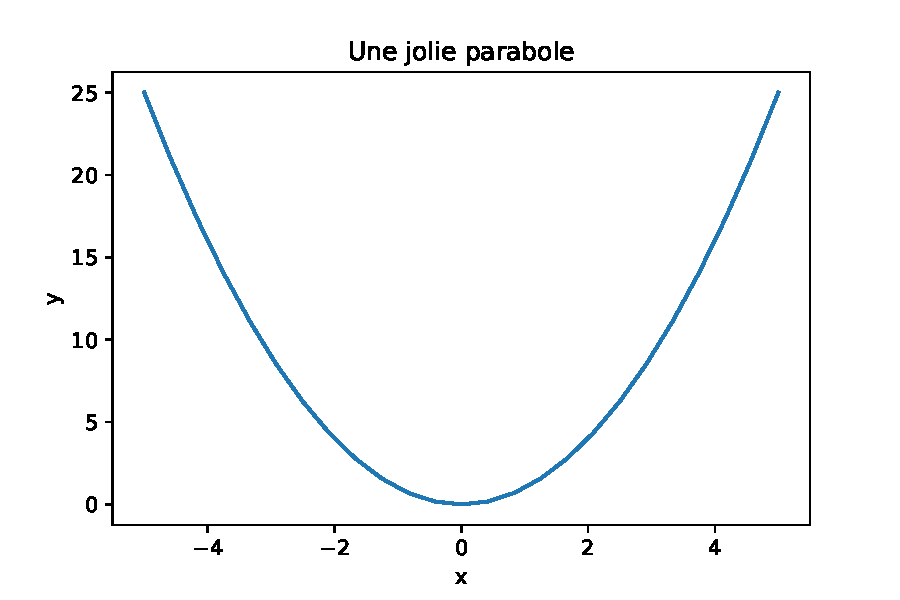
\includegraphics[width=0.5\textwidth]{imgs/parabole.pdf}
        \caption{Résultat obtenu avec le code ci-dessus.}
        \label{fig:parabole}
    \end{figure}
    
    Plus tout autre question concernant le code, ne l'oubliez jamais : Google est votre ami ! L'assistant aussi par ailleurs ;-)
    
    \pagebreak
    \pagestyle{nextpages}
    \part*{Exercices}
    
    \begin{exercice}[Calcul du BER d'un QAM-4]{1}
    
        L'objectif de cet exercice est de réussir à calculer le Bit Error Rate (BER), taux d'erreur en français, d'un signal et de voir son évolution en fonction du niveau de bruit, ou plutôt du Signal to Noise Ratio SNR.
        
        On considère donc la transmission d'une séquence de $N=\num{1e6}$ symboles QAM-4 :
        \begin{equation}
            x[k] = \pm 1 \pm j,
        \end{equation}
        avec $k=0,...,N$.
        
        Lors de l'envoi, le canal de transmission ajoute un bruit sur le signal de telle manière que le signal reçu, $y$, soit de la forme :
        \begin{equation}
            y[k] = x[k] + n[k],
        \end{equation}
        avec $n[k]$ le bruit à l'instant $k$.
        
        Ici, on modélise le bruit comme étant un bruit blanc gaussien, c.-à-.d une variable aléatoire suivant une distribution normale de moyenne nulle. Les symboles étant complexes, le bruit l'est tout autant. On notera donc $\sigma_n^2$ la variance du bruit complexe, et $\sigma_n^2/2$ la variance des parties réelles et imaginaires.
        
        Au récepteur, chaque symbole est décodé comme étant celui le plus proche de $y[k]$. On notera l'estimation du signal original $\hat{x}[k]$. Dans un monde idéal, sans bruit, on aura donc que $x[k]=\hat{x}[k]$ pour tout $k$. Le BER du signal est donc simplement le nombre de symboles erronés dans $\hat{x}[k]$ sur le nombre total de symboles.
        
        Finalement, on définit le SNR comme :
        \begin{equation}
            \text{SNR} = \frac{2}{\sigma_n^2}.
        \end{equation}
        
        \begin{enumerate}
            \item Générez la séquence $x[k]$ de manière aléatoire (voir \href{https://numpy.org/doc/stable/reference/random/generated/numpy.random.randint.html}{\py{numpy.random.randint}}).
            \item Générez la séquence $n[k]$ de bruit avec $\sigma_n^2 = \num{1e-2}$ (voir \href{https://numpy.org/doc/stable/reference/random/generated/numpy.random.randn.html}{\py{numpy.random.randn}}).
            \item Calculez les échantillons $y[k]$ et afficher les sur le diagramme de la constellation.
            \item Estimez le symbole d'origine $\hat{x}[k]$ sur base de cet échantillon.
            \item Calculez le BER.
            \item Refaites toutes ces étapes pour différents niveaux de bruits (conseil : utilisez \py{np.logspace(-2, 1, 25)}).
            \item Tracez la courbe du BER versus le SNR (conseil : utilisez \py{plt.semilogy(10 * np.log10(SNR), BER)}) et vérifiez que vous obtenez des résultats cohérents.
        \end{enumerate}
    
    \end{exercice}
    
    \begin{reponse}
        Une solution possible à l'exercice peut être visionnée dans ce \href{https://github.com/jeertmans/LELEC1930/blob/main/notebooks/seance4.ipynb}{Notebook}.
    \end{reponse}
    
    \begin{exercice}[Discrete Cosine Tranform]{2}
    
    \end{exercice}
    
    \begin{reponse}
        Une solution possible à l'exercice peut être visionnée dans ce \href{https://github.com/jeertmans/LELEC1930/blob/main/notebooks/seance4.ipynb}{Notebook}.
    \end{reponse}

\end{document}